\documentclass[11pt, a4paper]{article}

\usepackage[a4paper, width = 150 mm, top = 25 mm, bottom = 25 mm]{geometry}
\usepackage{amsfonts}
\usepackage{titlesec}
\usepackage{color}
\usepackage{graphicx}
\usepackage{subcaption}
\usepackage{verbatim}
\usepackage[style=apa,backend=biber, citestyle=authoryear, sorting=nyt]{biblatex}
\addbibresource{references.bib}


\title{Controlling Player Avatars in Game Worlds using Multi-Modal Input Systems}
\author{Charlie Lloyd-Buckingham}
\date{\today}


\newcommand{\addfigure}[1]
{\hfill 

\textcolor{red}{[Add Figure: #1]}

\hfill}



\newcommand{\addcitation}{\textcolor{red}{[Citation Need]}}
\newcommand{\ccite}[1]{(\citeauthor{#1}, \citeyear{#1})}
\newcommand{\cciteyear}[1]{(\citeyear{#1})}
\newcommand{\cciteauthor}[1]{(\citeauthor{#1})}
\newcommand{\reffig}[1]{Figure \ref{#1}}

\begin{document}

% Controlling Player Avatars in Game Worlds using Multi-Modal Input Systems
\maketitle



\pagebreak
\section{Acknowledgements}	
This is my acknowledgements.

\section{Abstract}	
My project is about....



\pagebreak
\tableofcontents				% - 300 Words



% Introducition and Context, Including Aim's and Objectives
\pagebreak
\section{Introduction}	
\subsection{Context}
Throughout the history of the games industry, game makers have been exploring new ways to deliver their players unique experiences. This has come in the forms of the narrative decisions within a game's story, stylistic decisions through the game's art and, as a focus for this paper, the interaction systems designed around the player's influence within a game's world. 

\hfill

On account of the digital nature of video games, as technology has evolved over the years, so too has the hardware and methods of interaction used within gaming consoles. Beginning in 1972 with the creation of the first home console, the Magnavox Odyssey, over the following years, video game console manufactures have continued to push the perceived boundaries of interactive entertainment. In 2006, Nintendo demonstrated the potential of a motion controlled input system with the Wii. Following this, other manufactures also began to expand into the technology, with Microsoft developing the Xbox Kinect and Sony the PlayStation Move. Nowadays, companies like Oculus and the HTC corporation are exploring the market of consumer virtual reality headsets with the Quest and Vive, while Nintendo is showing off new ways of using old technology with their Labo Toycon games. All of this has demonstrated that with the market's continued interest in new experiences, console manufactures and game developers will continue innovating new methods of interaction for their players.

\subsection{Research Problem}
There has also been a growing interest in the usage of electroencephalographic (EEG) and electromyographic (EMG) techniques being coupled with game engines for the purpose of research. The use of games in research has been invaluable for decades, due to the control gained over how a subject is stimulated throughout an experiment's lifetime. The act of reversing this dynamic and using these systems for the purpose of entertainment has also been explored \ccite{6518141}, however there is yet be any product viable for consumers to play. 

\subsection{Project Aims}
It is with this in mind, that this paper proposes to continue with the investigation into the viability of EEG, EMG, and other additional input modalities within video games. By acquiring data from all devices and combining them, the aim is for the creation of a single system capable of attaining and extracting meaningful interactions from it's users for control over aspects of game world. Along side this, two example games will also be constructed, these will be used to verify if the system is capable of performing it's tasks correctly and potentially demonstrate a working example from within a use-case environment.

\subsection{Project Objectives}
To get this system working, data from each device will need to be accessed live and streamed into the Unity game engine where a pre-trained artificial neural network (ANN) will be used to decipher a meaning suitable for the given game. From this the two games will be developed: the first will have the player use motor imagery to control the limbs of a virtual avatar; the second game will use the system measure the users state of mind, allowing for adaptive difficulty depending on the focus of the player.

% Review of Literature and / or Proffesional Practices
\pagebreak
\section{Research}	
\subsection{Literature Review}	% - 2000 Words
The usage of multi-modal input systems is not unheard of, almost all modern first person console shooters use the input controller's built in gyroscope, in addition to the right joystick to control the direction of the players camera. This multi-input system allows much more finesse when aiming, resulting in the players having a more enjoyable experience \ccite{toktacs2019evaluation}. In the work put forward by Silva and Amaral \cciteyear{da2014multimodal}, they demonstrate that the inclusion of a multi-modal input system compared to a uni-modal input system can make video games perceivably more enjoyable, ``it can be used to increase the feeling of empowerment on the player when using certain abilities, or to intentionally make in-game actions more difficult by demanding more physical effort from the player''. Though gyroscopic-assisted aiming is a more recent phenomenon, the concept of incorporating multiple input systems for singular interactions within gaming has been around for a while. Even back in 2009 with the release of `The Legend of Zelda: Spirit Tracks' \ccite{thelegendofzelda_spirittracks}, when using the flute, players would be required to both blow into the DS microphone and use the touch screen to play specific tones. This interaction could have very easily be performed by mapping tones to regions on the touch screen, or pairing each tone to a button on the Nintendo DS, much like how previous instruments in the franchise have been implemented, E.g. `The Legend of Zelda: Majoras Mask' \ccite{thelegendofzelda_majorasmask}. However, as stated by Silva, players could have a ``feeling of empowerment'' overcoming the set-pieces Nintendo designed, through this added multi-modal challenge.

\hfill

Before looking into EEG as a part of a larger multi-modal input system, a focus on how it has been used on its own within video gaming will be explored. Games using EEG most commonly occur in the form of serious games, defined by Alvarez and colleagues \cciteyear{alvarez2011introduction} as a video game that is ``intended to depart from the simple entertainment''. This refers to games built for research, education and rehabilitation. Whether this is just for providing an environment for the comparison between different electroencephalographs \ccite{liarokapis2014comparing}, evaluating a participant's emotions and satisfaction \ccite{vourvopoulos2013brain}, screening for early signs of mental illness \ccite{tarnanas2015comparison}, or cognitive rehabilitation \ccite{alchalcabi2017more}. 

The data captured from EEG can be used in a multitude of ways, depending on what is considered important for a given experiment. By using games it is then possible to focus on these targeted aspects of EEG: allowing for the invocation of responses necessary for measuring event related potentials \ccite{ahn2011using}, or to provide a real-time environment capable of demonstrating the changes in mental states \ccite{liarokapis2015examining} and motor-imagery \ccite{ndulue2019driving}. 

However, it is debated whether EEG technology is still in it's infancy. When investigating the current state of brain computer interfaces (BCIs) usability in the context of information transfer rates (ITR), Rashid and colleagues \cciteyear{rashid2020current} write ``In spite of the many outstanding breakthroughs that have been achieved in BCI research, some issues still need to be resolved... the existing BCIs offer somewhat poor ITR for any type of effectual BCI application'', while in Cattan's \cciteyear{cattan2021use} comparison, they state ``In practice, this means that BCIs are unusable in traditional inputs, such as in keyboards or mice''. To the contrary, EEG technology has already been used within for video games as an interactive medium: from modifying a game's difficulty based on the focus of the player with Tetris \ccite{liarokapis2015examining}; walking around the streets of Ancient Rome using motor-imagery in Rome Reborn \ccite{ndulue2019driving}; to piloting a space ship in Rock Evaders \ccite{ndulue2019driving}. EEG has shown its potential as a possible use for video game control.

\hfill

The usage of EMG within video games has also been quite extensive. EMG based serious games have permitted the research of various topics, from measuring arousal to stimuli using the muscles in the face \ccite{schuurink2008engagement}, to the effectiveness of myoelectric prosthesis training \ccite{bessa2020designing}. While their use outside of research has aided in the rehabilitation of patients, suffering: post injury \ccite{gutierrez2020serious} \ccite{schonauer2011full}; strokes \ccite{ghassemi2019development} and other medical disorders \ccite{labruyere2013requirements}. Though much more infrequent, entertainment focused EMG games do exist. In large part with they goal for allowing people with motor impairments to have the opportunities to play games, Kamau-Mugro \cciteyear{muguro2020development} states ``focusing on neck EMG, would give more control to individuals with hand disabilities or SCI [Spinal Cord Injury] patient as a control scheme or an entertainment interface''.

\hfill
  
Having investigated the viability of EEG and EMG as uni-modal input systems, an exploration into their combined usage alongside other additional input modalities can be performed. Though the appearance of entertainment based multi-modal EEG and EMG systems are infrequent, multi-modal serious games using EEG and EMG are a lot more common. An example of which is Sivanathans \cciteyear{sivanathan2014temporal} work on multi-modal EEG analysis, in which data from in-game events was coupled with the EEG input streams to allow for a greater understanding of the results. Though there isn't many instances of multi-modal EEG and EMG based video game systems, that isn't to say inspiration for these systems cannot come from elsewhere, the majority of research in which multi-modal EEG and EMG systems have been built for is in the development of consumer prosthetics \ccite{shi2019novel} and wheelchair controllers \ccite{carlson2013brain}. These systems pull from the data streams of EEG and EMG and by using eye-tracking, computer vision and inverse kinematics \ccite{mcmullen2013demonstration} are able to allow for finer control over hardware systems that on their own EEG and EMG wouldn't be able. By adopting a similar approach, these real world solutions can be used with virtual controllers instead. 







\pagebreak
\section{Methodology and Process}			% - 5100 Words

In this section, the design and implementation of both the system and example game will be discussed. The system, shown in \reffig{fig:system_diagram_:_generic}, will be devised to allow for the retrieval of real-time data from three input devices: the Emteq Pro, for sampling the EMG data; the eego sports, for sampling EEG data; and a compatible VR headset, for tracking player position and orientation. Following this, required data will pass them over a local network and, using machine learning, the system would construe a meaning from these inputs which was then used within the game.



\begin{figure}[h!]
	\centering
	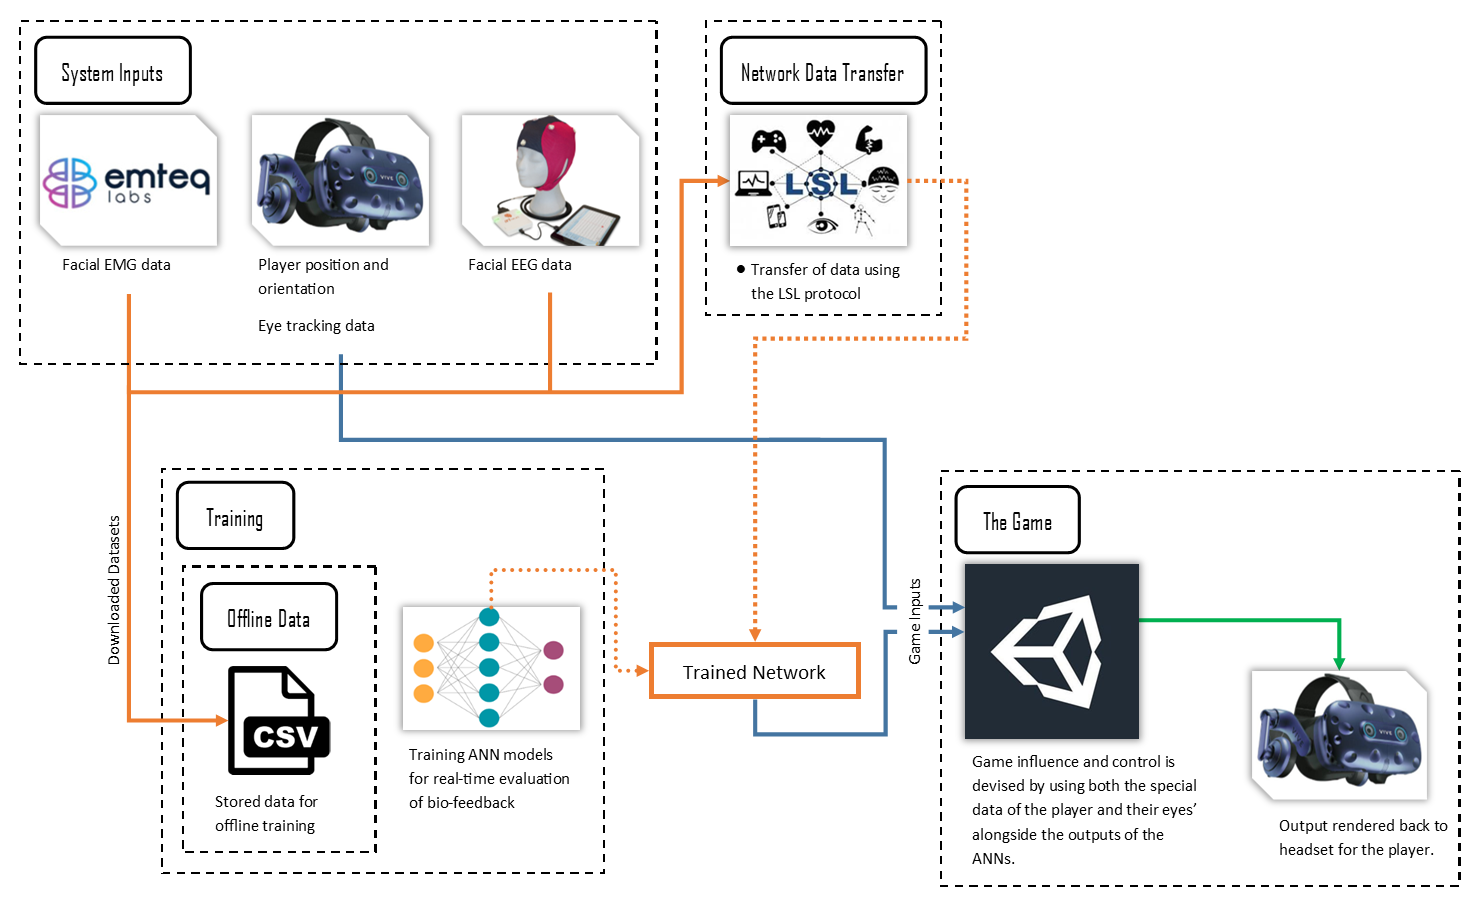
\includegraphics[width = 0.9 \linewidth] {[ Figures ]/System Diagram.png}
	\caption{System diagram: How input data from the specified technologies will be accessed and used within the game.}
	\label{fig:system_diagram_:_generic}
\end{figure}



The game was developed in the Unity 3D game engine, all technologies where integrated into the engine using C\#, and a variety of packages provided for Unity. The game itself consisted of a collection of two mini-games, both focusing on different aspects of how a system like this could be used in a real world consumer ready example. 

The first, \reffig{fig:the_game_1}, was a clone of the arcade game Breakout \addcitation{}, in which the player aim to break all blocks on the board by reflecting a ball into them using a paddle at the bottom of the play area. The intent with this part of the project was to allow for indirect influences of the player on the game world, in this case through difficulty scaling. This was done by classifying the players state of relaxation and concentration, increasing and decreasing the balls movement speed based what state the system deemed to be most likely.

The second mini-game, \reffig{fig:the_game_2}, was about repeating a randomised sequence of colours. The player would be tasked with repeating this sequence back, by activating crystals of the same colours in the same order. This mini-game was used to explore the concepts of motor-imagery based avatar control. This was accomplished by requiring the player to activate a crystals by lifting one of the avatars arms up. To accomplish this the player was required to think left-wards or right-wards and in doing so the avatar would begin lifting the chosen hand forwards. 



\begin{figure}[h!]
	\centering
	\begin{subfigure}[b]{0.45\linewidth}
		
\includegraphics[width = \linewidth] {[ Figures ]/Get Figure.png}
		\caption{Concentration based difficulty, Breakout mini-game.}
		\label{fig:the_game_1}
	\end{subfigure}
	\begin{subfigure}[b]{0.45\linewidth}
		
\includegraphics[width = \linewidth] {[ Figures ]/Get Figure.png}
		\caption{Motor imagery controlled, sequence mini-game.}
		\label{fig:the_game_2}
	\end{subfigure}
	\caption{The game.}
	\label{fig:the_game}
\end{figure}





%System Inputs
\subsection{System Inputs}	
Research into the different input methodologies demonstrated 

\addfigure{Zoom in of 'System Inputs' section of the diagram}

\subsubsection{EEG}	
The recording of live EEG data is accomplished by sampling voltage potentials across a users scalp using an array of sensors, these signals are then collated within an amplifier, such as the EEGO Sport, and accessed in the form of a stream of float channels, usually one channel for each of the sensors. The usages of this technology within the project will be specificity for motor imagery, and relaxation and concentration classification. Accessing this data live will be discussed in the networking part of this paper, however worth noting is that, due to the impractical nature of constant EEG tests, the large majority of this project was built around spoofing live EEG data using offline recordings.


\subsubsection{EMG}	
Similarly with EEG, EMG is the recording of the ambient voltage given from the activation of motor neurons. By placing these sensors across the certain regions of the body, models of muscular movements can be understood. The use of this technology within this project was focused around the eye, where it was used to detect blinking. This was to act as a way of stopping muscular interference within the EEG data caused by player blinks. Offline EMG data was also used in replacement for needing true live data.


\subsubsection{VR}	
Though this system was initially intended for the use of the HTC Vive Pro Eye, with Unity's XR Interaction Tool-kit package the specific headset used within the project is a bit less consequential. Using the this package, the tracking data accessed from a headsets can be very easily from a variety of different devices. However, headsets require that a project to be built for a specific platform, such as Android or Windows. With the intent of building this project for the HTC Vive however, the build platform can remain as Windows. In addition, this allowed for a mouse and keyboard solution to also be integrated into the project, to replace the inputs given via the headsets. This was important to do as it allowed for faster and less cumbersome testing of the solution. This replaced the headsets orientation tracking with a parametric based look function controlled via the mouses movement delta, as well as control over the paddle in breakout using the `A' and `D' keys, instead of inputs from the headsets controller.





%Network Data Transfer
\subsection{Network Data Transfer}	
%Unlike the data from VR headsets and the emteq pro, where access is easily given through Unity packages, accessing EEG data is more complicated through using the LSL protocol.
Unlike the direct access that VR headsets and the Emteq Pro gives to their data within Unity through the packages provided, accessing the EEG data can't be done so easily. The solution is the LSL protocol. 
% Explain what LSL is and why is useful before why using it here. OpenVibe Figure?
The EEGO Sport amplifier supports real-time writing of all data recorded during a session over a local network using the LSL protocol. LSL is designed to allow for near real-time access of data from anywhere on a local network. For this to work in Unity the 'liblsl-Csharp' package \addcitation{} was used, when using a non-standalone headset like the HTC Vive the Windows LSL .dll is required, while other headsets like the Pico Neo or the Oculus require their own Android .dll to allow for LSL to work within Unity. 

With the .dll's and the LSL.cs file is within the project, C\# scripts for writing to and reading from the network can be written. These retrieval scripts were written to now access EEG data in real time from within the game.





%Machine Learning
\subsection{Machine Learning}	
\subsubsection{Python}	
\subsubsection{Keras}	
\subsubsection{Keras Tuner}
\subsubsection{Baracuda}	


%The Games



Though this project is designed to work on a VR headset with real-time EEG and EMG data provided, testing resulted in building the project for Windows PC's with a mouse / keyboard input system, alongside offline EEG and EMG data.  


















\begin{comment}
\pagebreak
\subsection{Introduction to the project}
The project was created in the Unity game engine, the two mini-games chosen where a simple repeating sequence game and a implementation of the game Breakout \addcitation{}. The sequence game was chosen due to it not requiring accurate or high response inputs, this allowed it to be perfect for the possibly inaccurate readings of motor imagery. While breakout was chosen due to it's simplicity and ease for increasing game difficulty through the changing of ball speed. 

\subsubsection{Mini-game: Sequence}
In the repeating sequence game, players would be required to repeat back a sequence of colours shown to them by 'activating' similarly coloured crystals. This was done using a combination of 'Motor Imagery EEG' and EMG, where the player would be given control over an avatars arms by looking in a direction and thinking about moving one half of there body. This would trigger a response from the game, having there avatar reach forward and touch a crystal.

\addfigure %Add image of the minigame

\subsubsection{Mini-game: Breakout}
In Breakout, the player is given direct control of the paddle using the 'A' and 'D' on the keyboard. When the player is giving a lower level of focus the ball will increase its velocity, while the opposite is true when the player begins to focus more. Much like the original, the aim of the game is to destroy all the blocks.

\addfigure %Add image of the minigame

\pagebreak
\subsection{EEG and EMG }
\subsubsection{Keras and Keras Tuner}
To decipher the meaning given from the EEG and EMG data, the solution of a Neural Network was required. This was accomplished using a Python library called Keras, an interface library for Google's TensorFlow library. Motor Imagery data from \addcitation{}, was then downloaded, this data was originally in .edf format and was first converted to the .csv format for easier human readability, after which was then supplied to the networks for training. 

\hfill

This however gave some what lacklustre accuracy when used, so in addition the use of hyper-parameter optimisation was used. The library used in this project to do this was KerasTuner, the purpose of which was to search for the optimal design of a network: changing the types of activation functions, number of layers and size of these layers; to allow for a much more accurate model.

\addfigure %Add image of the networks training

\subsubsection{Barracuda}
After creating several reasonably accurate models using \addcitation{} and \addcitation{} data. The next step was to import these models into Unity. Unity has its own built in packages for Neural Networks, these being Unity Machine Learning Agents and Barracuda. The former focuses mainly on NPC AI, while the later can be used for almost any type of network, however required said network be in the .ONNX format. Due to the usage of this projects ANN's being classification based, Barracuda was the obvious choice, however the Keras produces networks of the .h5 format, as such a conversion was required. To do this, another python program was written to convert between .h5 and .ONNX models using the Keras2Onnx library. With this a script could finally be written within Unity to allow for the in-game real-time usage of these models.

\pagebreak
\subsection{LSL}
\subsubsection{Integration}
To receive the data from the input devices, the use of the LSL protocol was required. Specifically for this project the 'liblsl-Csharp' package \addcitation{} was used. This was imported into Unity and several scripts where then written to allow for the listening and broadcasting of different data types. To test whether this was working different devices on the network where then used to display the data using the 'Brain Vision LSL Viewer' application.

\addfigure %Add image of the position tracker LSL scripts.

\subsubsection{Online Data Spoofing}
With the cross-device communication working, the next stage was to create a script for spoofing potential online data. This would be used to see if the neural networks generated by Keras Tuner where working in the engine correctly. Offline data supplied by the dataset used previously from the network's training, though not used directly in it, was then attached to Unity through a script, in the format of .csv's. Each frame, this script would publish the next lines content over the network, allowing for faked online EEG and EMG data.

\hfill

\subsubsection{Testing the models}



\addfigure %Add image of the cube that moves for left and right.

\break
\begin{itemize}
  \item 1)	Setup of Unity enviroment for VR (Describe the game).
  \item 1.5) Show figure of game, and input devices
  \item 2)	Two Mini Games (Sequence) - Introduction
  \item 2.5) Show figure of devices,
  \item 3)	Two Mini Games (Breakout) - Introduction
  \item 2.5) Show figure of device and how they connect and are used,
  \item 4)	I began by using python - (tensor flow, keras) - to classify EEG data using motor imagery to decide between a left and right motion.
  \item 5)	To get a more accurate network I looked into KerasTuner, a hyper peramiter optimisation library for Keras.
  \item 6)	LSL streams used for aquiring and writing data.
  \item 7)	Offline processing and spoofing "online data" (reading CSV files) and writing the data over the LSL network.
  \item 8)	Combining Barracuda with LSL.
  \item 9)	Sequence games implementation.
  \item 10)	Breakouts implementation.
\end{itemize}
\end{comment}




\pagebreak
\section{Conclusion and Future Work}

\subsection{Conclusion}

\subsection{Future Work}			% - 300 Words



		% - 300 Words

\pagebreak
\printbibliography[notkeyword = software, title = References]

\pagebreak
\printbibliography[keyword = software, title = Software]

\end{document}
